\documentclass[conference]{IEEEtran}

\usepackage{cite}
\usepackage{amsmath,amssymb}
\usepackage{booktabs}
\usepackage{tikz}
\usepackage{url}
\usepackage{balance}
\usetikzlibrary{arrows.meta,positioning,shapes.geometric}

\begin{document}

\title{Scalable Fine-Grained eBPF Isolation through Hybrid Policy Verification}

\author{
\IEEEauthorblockN{Royal Dsouza}
\IEEEauthorblockA{
MCA Program\\
St. Aloysius University, Miri, India
}
}

\maketitle

\begin{abstract}
Multi-tenant cloud systems increasingly use extended Berkeley Packet Filter (eBPF) programs for networking, observability, and security while sharing a common Linux kernel. Fine-grained isolation policies can constrain helper usage, memory access, map operations, and other security-sensitive behavior, but policy verification based on symbolic execution can incur substantial end-to-end cost as feasible symbolic paths increase. This work investigates whether a lightweight abstract policy-analysis stage can safely discharge policy-compliant or policy-violating eBPF programs before invoking an expensive symbolic verifier, while retaining symbolic execution as a fallback for unresolved cases. We first reproduce and characterize a frozen KRAKENGUARD configuration through two baseline experiments. E1 evaluates a controlled micro-corpus with increasing compiled features, while E2 directly controls feasible symbolic path counts from 1 to 64. We then implement and evaluate a hybrid analyzer over a 24-program validation corpus containing provably compliant, uncertain compliant, provably violating, and symbolically discovered violation cases. In the tested corpus, the abstract stage discharged 12 of 24 programs (50.0\%) with zero false SAFE and zero false VIOLATION decisions. Across 432 E4 executions, hybrid verification reduced the overall median end-to-end time from 694.28 ms to 382.32 ms, corresponding to 45.53\% median per-program savings. These findings provide experimental evidence that selective abstract discharge can reduce the amount of symbolic verification required for the evaluated eBPF isolation workloads. The conclusions are bounded to the tested corpus, path range, frozen verifier, policy, and execution environment.
\end{abstract}

\begin{IEEEkeywords}
eBPF, multi-tenant cloud security, eBPF isolation, symbolic execution, abstract analysis, policy verification, KRAKENGUARD
\end{IEEEkeywords}

\section{Introduction}

Cloud infrastructure increasingly consolidates multiple workloads on shared Linux hosts. This multi-tenant model improves utilization, but it also means that security mechanisms operating inside the kernel must distinguish what one tenant is authorized to do from what another tenant is allowed to do. Extended Berkeley Packet Filter (eBPF) provides a programmable interface for networking, tracing, observability, and security, making it attractive for cloud-native infrastructure. At the same time, its kernel-level execution model makes isolation and policy enforcement important security concerns.

The Linux eBPF verifier provides a fundamental safety gate, but verifier safety and fine-grained tenant policy compliance are different questions. A program may satisfy verifier safety requirements while still violating a tenant-specific policy governing helper calls, maps, memory, return values, or interactions with other programs. Recent systems have therefore explored fine-grained policy analysis and related verifier-assurance mechanisms. KRAKENGUARD, for example, uses symbolic analysis to reason about fine-grained eBPF isolation policies and identifies symbolic path and expression growth as an important scalability concern \cite{patel2026krakenguard}. Other recent work addresses verifier precision through proof-guided refinement, verifier-resilient execution, verifier testing, tenant virtualization, and resource isolation \cite{sun2025bcf,sun2025aee,lyu2025veritas,zhang2026vbpf,carin2026peer}.

This work focuses on a narrower question within that broader multi-tenant security problem: whether expensive symbolic policy verification can be invoked selectively rather than universally. The central research question is:

\begin{quote}
Can fine-grained eBPF isolation policies be checked with predictable cost by combining inexpensive abstract analysis with selective symbolic execution?
\end{quote}

The proposed approach places a lightweight abstract policy analyzer before symbolic verification. The analyzer uses a conservative three-valued decision model: \textsc{Safe}, \textsc{Violation}, or \textsc{Unknown}. A proven safe program is accepted, a proven violation is rejected, and an unresolved program is forwarded to the frozen symbolic verifier. The design is intentionally fail-closed: lack of proof is not treated as safety.

The contribution of this paper is therefore not a replacement for the Linux verifier or KRAKENGUARD. Instead, the contribution is an experimentally evaluated verification workflow that attempts to avoid unnecessary symbolic verification while preserving symbolic fallback for unresolved programs.

The paper makes four contributions:
\begin{enumerate}
    \item We characterize the cost behavior of a frozen KRAKENGUARD configuration using controlled program-feature and symbolic-path experiments.
    \item We design a conservative abstract policy-analysis stage with explicit \textsc{Safe}, \textsc{Violation}, and \textsc{Unknown} outcomes.
    \item We evaluate selective discharge and hybrid end-to-end performance on a 24-program eBPF corpus.
    \item We report the observed performance and correctness results together with explicit experimental boundaries and provenance controls.
\end{enumerate}

\section{Background and Motivation}

\subsection{eBPF in Multi-Tenant Infrastructure}

eBPF allows user-supplied programs to execute at selected kernel hooks. In cloud infrastructure, XDP is one relevant hook because it enables high-performance packet processing close to the network receive path. The same programmability that makes eBPF useful also creates an isolation requirement: a tenant-specific program must remain within the authority defined for that tenant.

The security problem can be expressed as a policy decision over an eBPF program $P$ and policy $\Pi$:
\[
    V(P,\Pi) \in \{\mathrm{COMPLIANT},\mathrm{VIOLATION}\}.
\]
The policy may constrain operations such as helper calls, map accesses, memory behavior, or return values. The important distinction is that policy compliance is workload- and tenant-specific, whereas verifier safety is a more general property of whether the program is safe to execute under the kernel's verifier rules.

\subsection{Symbolic Policy Verification}

KRAKENGUARD provides a relevant baseline for fine-grained eBPF isolation. Its verification pipeline lifts eBPF bytecode into an intermediate representation, resolves helpers and other symbols, constructs a verification harness, and uses KLEE-based symbolic execution to explore policy-relevant behavior \cite{patel2026krakenguard}. This makes symbolic execution useful for cases where the policy decision depends on values that cannot be determined by simple local inspection.

The drawback is that symbolic execution can require exploration of multiple feasible execution paths. If a program has $P$ feasible paths, the symbolic workload can increase as $P$ increases. The exact relationship is workload dependent; this paper does not assume a universal asymptotic complexity. Instead, E2 experimentally controls path growth in a synthetic family.

\subsection{Why a Hybrid Approach?}

A verifier that sends every program directly to symbolic execution pays the complete symbolic pipeline cost even when the policy decision is already obvious from the program's compiled structure. A conservative abstract analyzer can sometimes prove that a forbidden action is unreachable or that all reachable policy-relevant operations are compliant.

The key design principle is therefore:
\begin{equation}
H(P,\Pi)=
\begin{cases}
\mathrm{ACCEPT}, & A(P,\Pi)=\mathrm{SAFE},\\
\mathrm{REJECT}, & A(P,\Pi)=\mathrm{VIOLATION},\\
V_{\mathrm{sym}}(P,\Pi), & A(P,\Pi)=\mathrm{UNKNOWN}.
\end{cases}
\end{equation}
Here, $A$ is the abstract analyzer and $V_{\mathrm{sym}}$ is the authoritative symbolic verifier. The hybrid method does not claim that symbolic execution becomes intrinsically faster. Its potential benefit comes from avoiding symbolic execution entirely for programs that the abstract stage can decide.

\section{Related Work}

Recent eBPF research covers several dimensions of the security and isolation problem. KRAKENGUARD directly addresses fine-grained eBPF isolation using symbolic analysis and serves as the primary baseline for this study \cite{patel2026krakenguard}. BCF applies proof-guided abstraction refinement to improve verifier precision while constraining kernel complexity \cite{sun2025bcf}. Approximation Enforced Execution investigates runtime enforcement for untrusted Linux kernel extensions and changes the assumptions around verifier enforcement \cite{sun2025aee}. Veritas/SpecCheck uses specification-based testing to detect eBPF verifier misbehavior \cite{lyu2025veritas}.

Multi-tenant execution isolation is also being investigated independently of policy verification. vBPF explores eBPF virtualization and tenant/state isolation \cite{zhang2026vbpf}, while PeeR addresses scheduling and resource isolation for latency-critical eBPF applications \cite{carin2026peer}. BPF Token changes the delegation model for BPF operations through user-namespace-bound BPF filesystems \cite{bpftoken}. SeaBee addresses protection of security-critical eBPF infrastructure against privileged tampering \cite{seabee}.

These systems motivate the broader multi-tenant security context but do not make them interchangeable baselines for the specific policy-verification experiment in this paper. In particular, the present work evaluates a hybrid verification strategy against a frozen KRAKENGUARD policy-analysis configuration rather than proposing a new BPF namespace, virtualization layer, scheduler, or verifier.

\section{Research Problem and Hypotheses}

The research problem is to reduce unnecessary symbolic policy-verification work without converting uncertainty into an unsafe decision.

The primary research question is:
\begin{quote}
Can inexpensive abstract policy analysis discharge policy-safe eBPF programs before symbolic execution, while selectively forwarding unresolved programs to symbolic verification?
\end{quote}

The evaluation is divided into two logical questions. First, can the abstract stage safely classify a useful subset of programs? Second, does avoiding symbolic verification reduce complete end-to-end verification cost?

The Phase 5 hypotheses are:
\begin{itemize}
    \item \textbf{H5-C: Correctness.} Abstractly discharged final decisions agree with the frozen symbolic reference on the validation corpus.
    \item \textbf{H5-COV: Selective discharge.} A measurable subset of the corpus can be classified without symbolic fallback.
    \item \textbf{H5-P: End-to-end cost.} Hybrid verification reduces complete verification time when abstract-analysis cost plus any required fallback cost is lower than symbolic-only verification.
    \item \textbf{H5-S: Fallback scaling.} Fallback amount and cost can be characterized as symbolic path complexity increases.
\end{itemize}

\section{Hybrid Verification Design}

\subsection{Architecture}

The system is intentionally simple:

\begin{figure}[t]
\centering
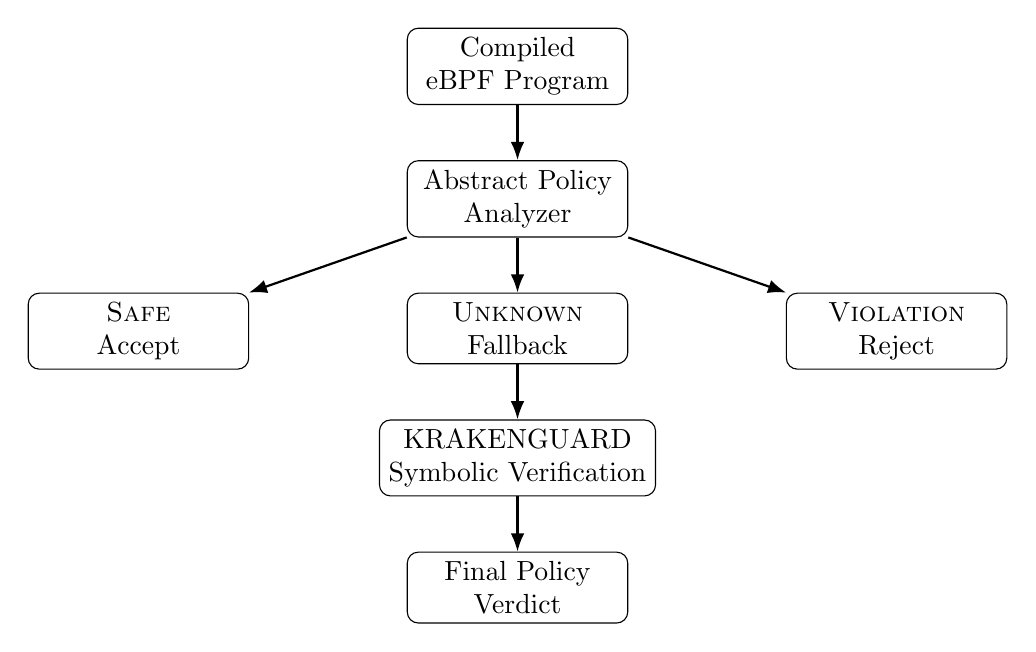
\begin{tikzpicture}[
node distance=7mm and 7mm,
box/.style={draw, rounded corners, align=center, minimum width=28mm, minimum height=8mm},
arrow/.style={-{Latex}, thick}
]
\node[box] (p) {Compiled\\eBPF Program};
\node[box, below=of p] (a) {Abstract Policy\\Analyzer};
\node[box, below left=of a, xshift=-13mm] (s) {\textsc{Safe}\\Accept};
\node[box, below=of a] (u) {\textsc{Unknown}\\Fallback};
\node[box, below right=of a, xshift=13mm] (v) {\textsc{Violation}\\Reject};
\node[box, below=of u] (k) {KRAKENGUARD\\Symbolic Verification};
\node[box, below=of k] (f) {Final Policy\\Verdict};
\draw[arrow] (p)--(a);
\draw[arrow] (a)--(s);
\draw[arrow] (a)--(u);
\draw[arrow] (a)--(v);
\draw[arrow] (u)--(k);
\draw[arrow] (k)--(f);
\end{tikzpicture}
\caption{Hybrid fine-grained eBPF policy-verification pipeline.}
\label{fig:architecture}
\end{figure}

The analyzer operates on the compiled eBPF object and its control-flow graph rather than relying only on source-level C syntax. It tracks reachability, selected integer facts, policy conditions, helper access, map access, memory ranges, return values, and analysis status.

\subsection{Three-Valued Abstract Decision}

The analyzer returns exactly one of three abstract decisions:
\begin{itemize}
    \item \textsc{Safe}: every reachable abstract state is proven policy compliant.
    \item \textsc{Violation}: a policy-forbidden action is proven reachable.
    \item \textsc{Unknown}: the available abstract domain cannot prove compliance or violation.
\end{itemize}

The distinction between \textsc{Unknown} and \textsc{Safe} is fundamental. Unsupported instructions, unknown helper identities, unresolved map identity or access mode, insufficient memory proofs, and unresolved branch conditions conservatively produce \textsc{Unknown}. A syntactic occurrence of a forbidden operation is not sufficient for \textsc{Violation} unless its reachability is established.

\subsection{Fail-Closed Semantics}

The analyzer is designed around a one-sided safety requirement: an abstract analysis failure must reduce precision, not increase authority. Therefore:
\[
    \mathrm{UNKNOWN} \not\Rightarrow \mathrm{SAFE}.
\]
Only the symbolic fallback can resolve an unresolved case. This design also makes the hybrid system compatible with the role of KRAKENGUARD as the authoritative reference for the experiments.

\section{Experimental Methodology}

\subsection{Frozen Baseline and Environment}

All experiments use a frozen KRAKENGUARD revision:
\[
\texttt{e7bd84005b304c5a10efcdb04914d1882b3cccf7}.
\]
The fixed policy used by E1 and Phase 5 has SHA-256:
\[
\texttt{270403272d736ae7aee2ceda3bf8d088b6ac0cb476bb99ce0218dd8f33c3c603}.
\]

The experimental environment is:
\begin{itemize}
    \item Linux kernel 7.2.3-arch1-2, x86\_64;
    \item AMD Ryzen 5 5600H, 12 logical cores;
    \item approximately 7.1 GiB RAM;
    \item Clang/LLVM 22.1.8;
    \item BPF target with \texttt{-mcpu=v1};
    \item optimization \texttt{-O2 -g};
    \item XDP hook type;
    \item Docker-based KRAKENGUARD artifact with immutable image digest \texttt{sha256:9633a6922518589803a4c9b8123d0549e54b5f57c1d04f9e383e822fd9ae3bd4}.
\end{itemize}

The compiler flags were \texttt{-target bpf -mcpu=v1 -D\_\_TARGET\_ARCH\_x86 -O2 -g} with the required system include path.

\subsection{E1: Program Complexity Scaling}

E1 evaluates how end-to-end KRAKENGUARD cost changes across eight synthetic XDP micro-programs while keeping policy and environment fixed. Each program was run for two warmups and seven measured repetitions, for 72 total executions.

The compiled corpus ranged from a 2-instruction minimal XDP program to a 20-instruction program combining branches, helpers, and a map. The measured median wall times were:

\begin{table}[t]
\centering
\caption{E1 median end-to-end verification time.}
\label{tab:e1}
\begin{tabular}{lrrr}
\toprule
Program & Instructions & Paths & Median (ms)\\
\midrule
P0 & 2  & 1 & 681.82\\
P1 & 5  & 1 & 679.87\\
P2 & 4  & 1 & 677.55\\
P3 & 18 & 1 & 672.43\\
P4 & 6  & 1 & 688.57\\
P5 & 11 & 1 & 692.90\\
P6 & 17 & 1 & 686.70\\
P7 & 20 & 2 & 707.61\\
\bottomrule
\end{tabular}
\end{table}

P0--P3 remained nearly flat despite a large increase in compiled instruction count. P4 exhibited one genuine timing spike, which was retained rather than removed. E1 therefore indicates that raw instruction count alone does not explain the observed end-to-end cost in this small regime. Feature-dependent symbolic behavior and fixed pipeline overhead are separate dimensions.

\subsection{E2: Controlled Symbolic Path Scaling}

E2 isolates feasible symbolic path growth more directly. The controlled program family produced 1, 2, 4, 8, 16, 32, and 64 feasible KLEE paths. Each level used two warmups and seven measured repetitions, for 63 total executions and 49 measured observations.

\begin{table}[t]
\centering
\caption{E2 verification cost versus observed feasible symbolic paths.}
\label{tab:e2}
\begin{tabular}{rrr}
\toprule
Paths & Median (ms) & Mean (ms)\\
\midrule
1  & 746.14  & 757.28\\
2  & 749.93  & 752.64\\
4  & 762.77  & 770.22\\
8  & 789.88  & 789.19\\
16 & 853.02  & 854.79\\
32 & 973.44  & 972.45\\
64 & 1231.16 & 1266.86\\
\bottomrule
\end{tabular}
\end{table}

The median increased by approximately 65.0\% from one path to 64 paths. A linear fit in the tested regime was approximately:
\[
T(P) \approx 740\ \mathrm{ms} + 7.6\ \mathrm{ms}\cdot P,
\]
with $R^2>0.999$ for the measured points. This is an empirical model for the tested family, not a claim of universal asymptotic complexity. E2 establishes the motivation for reducing the number of programs that require symbolic verification.

\subsection{Phase 5 Corpus}

The Phase 5 validation corpus contains 24 programs divided equally into four categories:
\begin{itemize}
    \item \textbf{A:} abstractly provable compliant, 6 programs;
    \item \textbf{B:} abstractly uncertain but symbolically compliant, 6 programs;
    \item \textbf{C:} abstractly provable violation, 6 programs;
    \item \textbf{D:} abstractly uncertain and symbolically violating, 6 programs.
\end{itemize}

This structure separates easy cases from cases that intentionally require the symbolic fallback.

\subsection{E3: Selective Discharge and Correctness}

E3 evaluates whether the abstract stage can classify a useful subset and whether its discharged decisions agree with the frozen symbolic reference. Each of the 24 programs was evaluated with two warmups and seven measured repetitions, producing 216 executions.

The primary endpoint is:
\[
D=\frac{N_{\mathrm{SAFE}}+N_{\mathrm{VIOLATION}}}{N_{\mathrm{total}}}.
\]

A correct hybrid decision is defined relative to the authoritative KRAKENGUARD result. The experiment requires zero false SAFE and zero false VIOLATION decisions; false UNKNOWN is acceptable because it invokes the fallback.

\subsection{E4: End-to-End Performance}

E4 compares two complete pipelines:
\begin{align}
T_{\mathrm{symbolic}} &= T_{\mathrm{KRAKENGUARD}},\\
T_{\mathrm{hybrid}} &=
\begin{cases}
T_{\mathrm{abstract}}, & \text{if discharged},\\
T_{\mathrm{abstract}}+T_{\mathrm{fallback}}, & \text{otherwise}.
\end{cases}
\end{align}

Each of the 24 programs was evaluated under both conditions, with two warmups and seven measured repetitions per condition. The total was therefore $24\times2\times9=432$ executions. Conditions were interleaved using deterministic randomization with seed 42. The primary endpoint is paired per-program median end-to-end wall time.

\subsection{E5: Fallback Scaling}

E5 examines how the hybrid workflow behaves across observed symbolic path strata. Reachable strata were 1, 2, 4, 8, 16, and 32. The 64-path stratum was unreachable for eligible Phase 5 programs and is therefore not reported as an observed result.

The experiment reports abstract time, fallback time, total hybrid time, and fallback fraction. It does not assume that the abstract analyzer accelerates symbolic execution itself. Its intended benefit is elimination of unnecessary symbolic invocations.

\section{Results}

\subsection{E3: Abstract Discharge}

The abstract analyzer discharged 12 of 24 programs:
\[
D=\frac{12}{24}=50.0\%.
\]
The Wilson score 95\% interval for this proportion is 31.4--68.6\%.

The category results were:

\begin{table}[t]
\centering
\caption{E3 discharge and correctness results.}
\label{tab:e3}
\begin{tabular}{lrrrr}
\toprule
Category & Count & Discharged & Rate & Result\\
\midrule
A & 6 & 6 & 100\% & SAFE\\
B & 6 & 0 & 0\% & UNKNOWN\\
C & 6 & 6 & 100\% & VIOLATION\\
D & 6 & 0 & 0\% & UNKNOWN\\
\midrule
Total & 24 & 12 & 50\% & ---\\
\bottomrule
\end{tabular}
\end{table}

All 24 final outcomes agreed with the KRAKENGUARD reference. There were zero false SAFE decisions and zero false VIOLATION decisions. Categories B and D were deliberately retained as \textsc{Unknown} by the abstract stage and therefore exercised the fallback path.

\subsection{E4: Hybrid Versus Symbolic-Only}

E4 produced 432 executions with zero timeouts, zero failures, and zero correctness mismatches in the recorded matrix. The overall median end-to-end time was 694.28 ms for symbolic-only verification and 382.32 ms for hybrid verification.

The median per-program savings were:
\[
S=1-\frac{T_{\mathrm{hybrid}}}{T_{\mathrm{symbolic}}}=45.53\%.
\]

\begin{table}[t]
\centering
\caption{E4 category-level performance.}
\label{tab:e4}
\begin{tabular}{lrrrr}
\toprule
Category & Fallback & Sym. (ms) & Hybrid (ms) & Savings\\
\midrule
A & 0.0 & 684.36 & 37.54 & 94.5\%\\
B & 1.0 & 727.34 & 765.75 & -4.8\%\\
C & 0.0 & 683.52 & 39.55 & 94.2\%\\
D & 1.0 & 700.96 & 735.89 & -5.1\%\\
\bottomrule
\end{tabular}
\end{table}

The result is driven by the discharged programs. Categories A and C together represent 50\% of the corpus and avoid symbolic verification entirely. Their hybrid medians are approximately 38--40 ms, compared with approximately 684 ms for symbolic-only verification. In contrast, B and D require fallback and therefore incur a small additional abstract-analysis cost, producing a modest regression relative to symbolic-only.

The 45.53\% figure is consequently an end-to-end workflow result, not a claim that KRAKENGUARD itself became 45.53\% faster.

\subsection{E5: Fallback Scaling}

\begin{table}[t]
\centering
\caption{E5 observed path strata.}
\label{tab:e5}
\begin{tabular}{rrrrr}
\toprule
Paths & Programs & Discharged & Fallback & Hybrid (ms)\\
\midrule
1  & 12 & 12 & 0\%   & 39.12\\
2  & 4  & 0  & 100\% & 731.33\\
4  & 2  & 0  & 100\% & 749.73\\
8  & 2  & 0  & 100\% & 768.28\\
16 & 2  & 0  & 100\% & 781.84\\
32 & 2  & 0  & 100\% & 852.68\\
64 & 0  & 0  & N/A   & N/A\\
\bottomrule
\end{tabular}
\end{table}

At one feasible path, all eligible programs in categories A and C were discharged without symbolic fallback. At higher observed strata, the Phase 5 corpus contained unresolved programs whose dynamic return conditions or branch-dependent policy behavior required KRAKENGUARD. Fallback time increased from approximately 696 ms at two paths to approximately 810 ms at 32 paths for the representative strata.

These observations are consistent with the E2 finding that symbolic work becomes increasingly costly as feasible path count increases. However, E5 does not establish a universal scaling law for the hybrid system.

\section{Discussion}

The experiments form a progression from baseline characterization to selective verification.

E1 shows that small increases in compiled instruction count do not necessarily translate into proportional increases in end-to-end policy-verification time. The pipeline contains substantial fixed work, including lifting, intermediate-representation processing, harness construction, compilation, linking, and verifier startup. This makes raw program length an incomplete predictor of cost in the tested regime.

E2 isolates a different factor. When feasible symbolic path count is deliberately increased, end-to-end verification time increases substantially. The controlled family therefore exposes a cost dimension that E1 only weakly exercised. The result motivates an optimization that does not attempt to make symbolic execution universally cheaper: instead, the system should avoid invoking symbolic execution when a cheaper analysis can already prove the policy result.

E3 demonstrates that this approach is possible for a meaningful subset of the tested corpus. The abstract analyzer discharged exactly the categories constructed to be abstractly decidable, while conservatively returning \textsc{Unknown} for the categories designed to require symbolic reasoning. The absence of false SAFE and false VIOLATION decisions is particularly important because the security cost of an incorrect SAFE decision is qualitatively different from the cost of an unnecessary fallback.

E4 provides the main end-to-end performance result. The hybrid workflow reduces the overall median time because half of the tested programs terminate after the abstract stage. The fallback cases do not become faster; they become slightly slower because the abstract stage adds overhead before symbolic verification. Therefore, the benefit depends on the proportion of workloads that can be safely discharged.

This leads to an important interpretation of the research contribution. The proposed method is not a universal replacement for symbolic verification. It is a selective front-end whose value depends on the availability of policy decisions that can be proven cheaply. The \textsc{Unknown} outcome is therefore a feature of the design rather than a failure state.

\section{Threats to Validity and Limitations}

Several limitations bound the conclusions.

\subsection{Corpus Scope}
The Phase 5 corpus contains 24 synthetic, policy-directed XDP programs. It is useful for controlled evaluation of the decision categories but is not representative of all production eBPF workloads. Large programs, complex parsers, large maps, tail calls, loops, and application-specific policies may exhibit different behavior.

\subsection{Reference Oracle}
Correctness is measured against the frozen KRAKENGUARD configuration. Agreement with a reference implementation establishes consistency with that implementation; it does not independently prove universal correctness of KRAKENGUARD.

\subsection{Environment}
All measurements were collected on one host, one kernel version, one compiler version, one XDP configuration, one frozen KRAKENGUARD revision, and one fixed policy. Results may differ on other systems.

\subsection{Path Range}
E2 experimentally covers 1--64 feasible paths. E5 reaches only 1--32 paths for eligible Phase 5 programs; the 64-path Phase 5 stratum was unreachable. No claim is made about behavior beyond these ranges.

\subsection{Measurement Scope}
Wall time is measured for the complete verification workflow. Client-process CPU time is not treated as equivalent to verifier wall time. Memory scaling and detailed solver-time scaling are not used as primary conclusions because they were not consistently exposed by the frozen pipeline.

\subsection{Generalization}
The 50.0\% discharge rate is a property of the evaluated 24-program corpus. It must not be interpreted as the fraction of arbitrary eBPF programs that can be discharged. Similarly, the 45.53\% savings figure is an observed corpus-level result and not a universal performance guarantee.

\section{Reproducibility and Provenance}

The experiments preserve the major controls needed to reproduce the evaluated configuration. The KRAKENGUARD source revision, policy hash, compiler, kernel, architecture, hook type, compiler flags, container image digest, corpus metadata, and raw execution artifacts are recorded in the repository.

The Phase 5 execution evidence is associated with the recovered execution state rooted at commit \texttt{0e1d96cf13574222e58de349ce885b28b6e0ac9d}; the recovered evidence tree was committed at \texttt{33c1fc6f3fd40555cc4c3483803d6d01c84e50b4}. E3 contains 216 records, E4 contains 432 records, and E5 is derived from preserved E4 telemetry for the reachable path strata.

The repository also records correction and validation artifacts documenting the fail-closed analyzer semantics, frozen policy resolution, environment preflight, and fallback verification. These artifacts are part of the reproducibility record and should be consulted together with the raw experiment data.

\section{Conclusion and Future Work}

This paper investigated whether fine-grained eBPF isolation policy verification can reduce unnecessary symbolic execution by placing a conservative abstract analyzer before a symbolic verifier.

The baseline experiments established two useful observations. First, small increases in compiled program features produced relatively stable end-to-end cost in the tested micro-corpus. Second, directly controlled feasible symbolic path growth from 1 to 64 paths produced a substantial increase in verification time. Together, these observations motivate reducing the number of workloads that reach symbolic verification rather than relying only on program-size metrics.

The Phase 5 evaluation then demonstrated selective discharge on a 24-program corpus. The abstract stage discharged 12 programs, corresponding to 50.0\%, while producing zero false SAFE and zero false VIOLATION decisions against the frozen KRAKENGUARD reference. Across 432 E4 executions, the hybrid workflow reduced the overall median end-to-end time from 694.28 ms to 382.32 ms, yielding 45.53\% median per-program savings. The improvement comes from eliminating symbolic verification for discharged programs; unresolved programs still require the fallback and incur its cost.

The resulting evidence supports the narrower claim that selective abstract policy analysis can reduce symbolic-verification work for the evaluated eBPF isolation corpus under the frozen experimental configuration. It does not establish universal performance, universal discharge coverage, or production-scale behavior.

Future work should evaluate larger and less synthetic eBPF workloads, richer policy predicates, additional hook types, larger symbolic path regimes, and independent symbolic-verification references. A particularly important direction is adaptive abstract-domain refinement: rather than expanding the abstract domain indiscriminately, future systems could identify the policy predicates responsible for \textsc{Unknown} results and selectively refine only those cases.

\section*{Acknowledgment}
The author thanks the maintainers and authors of the open-source eBPF analysis infrastructure used as experimental baselines. The experiments and analysis reported here are intended as a research evaluation and not as a production security guarantee.

\balance
\bibliographystyle{IEEEtran}
\bibliography{references}

\end{document}
